\documentclass[11pt,a4paper]{article}

\usepackage[margin=2.4cm]{geometry}
\usepackage{graphicx}
\usepackage[hidelinks]{hyperref}
\usepackage{booktabs}
\usepackage{enumitem}
\usepackage{float}
\usepackage{xcolor}
\usepackage{url}

\setlength{\parskip}{0.7em}
\setlength{\parindent}{0pt}
\graphicspath{{../figures/}}

\title{\textbf{Air Quality, Socio-economic Disadvantage and Urban Exposure Patterns in Victoria}}
\author{}
\date{}

\begin{document}
\maketitle

\section*{Abstract}

This project analyses 2024 air-quality exposure patterns in Victoria, Australia, with a focused socio-economic analysis for Greater Melbourne. It combines EPA Victoria hourly monitoring records, Australian Bureau of Statistics SEIFA 2021 indexes, and ASGS 2021 SA2 boundary data. The workflow cleans and validates hourly observations, constructs station-level and time-based summaries, estimates SA2-level exposure surfaces within Greater Melbourne, and compares those exposure estimates against multiple SEIFA dimensions. The main finding is that the exposure-equity story is pollutant-specific: PM2.5 is elevated in several inner and relatively advantaged areas, while NO2 and O3 show stronger relationships with education and occupation disadvantage.

\section{Data}

The project uses three public data sources:

\begin{itemize}[leftmargin=*]
  \item EPA Victoria / DataVic hourly air-quality data for all AirWatch sites in 2024.
  \item ABS SEIFA 2021 SA2 indexes, including IRSD, IRSAD, IER and IEO.
  \item ABS ASGS Edition 3 SA2 digital boundary files.
\end{itemize}

The local raw data contain 816,133 hourly air-quality records across 15 monitoring stations. The processed data include 15 station records, 40 station-by-pollutant summary rows, 6,552 weekday-hour pattern rows, 361 Greater Melbourne SA2 GeoJSON features, and 16 pollutant-SEIFA correlation rows using 356 SA2s with complete values.

\section{Pre-processing Workflow}

The Python workflow performs the following steps:

\begin{enumerate}[leftmargin=*]
  \item Reads the local AirWatch Excel workbook, SEIFA workbook and SA2 shapefile.
  \item Keeps 2024 observations for PM2.5, PM10, NO2, O3, SO2 and CO.
  \item Parses local timestamps and derives month, date, weekday, hour and season.
  \item Keeps validated observations only.
  \item Removes duplicate records using station, local time, AEST time and pollutant as the duplicate key.
  \item Builds station-level annual, seasonal, monthly and weekday-hour summaries.
  \item Joins monitoring stations to SA2 boundaries.
  \item Estimates Greater Melbourne SA2 exposure values using inverse distance weighting from metropolitan stations.
  \item Calculates exceedance-day counts and Spearman correlations against SEIFA scores.
\end{enumerate}

The spatial analysis is deliberately restricted to Greater Melbourne. The full Victoria monitoring network is too sparse for a credible statewide continuous exposure surface.

\section{Temporal Patterns}

\begin{figure}[H]
  \centering
  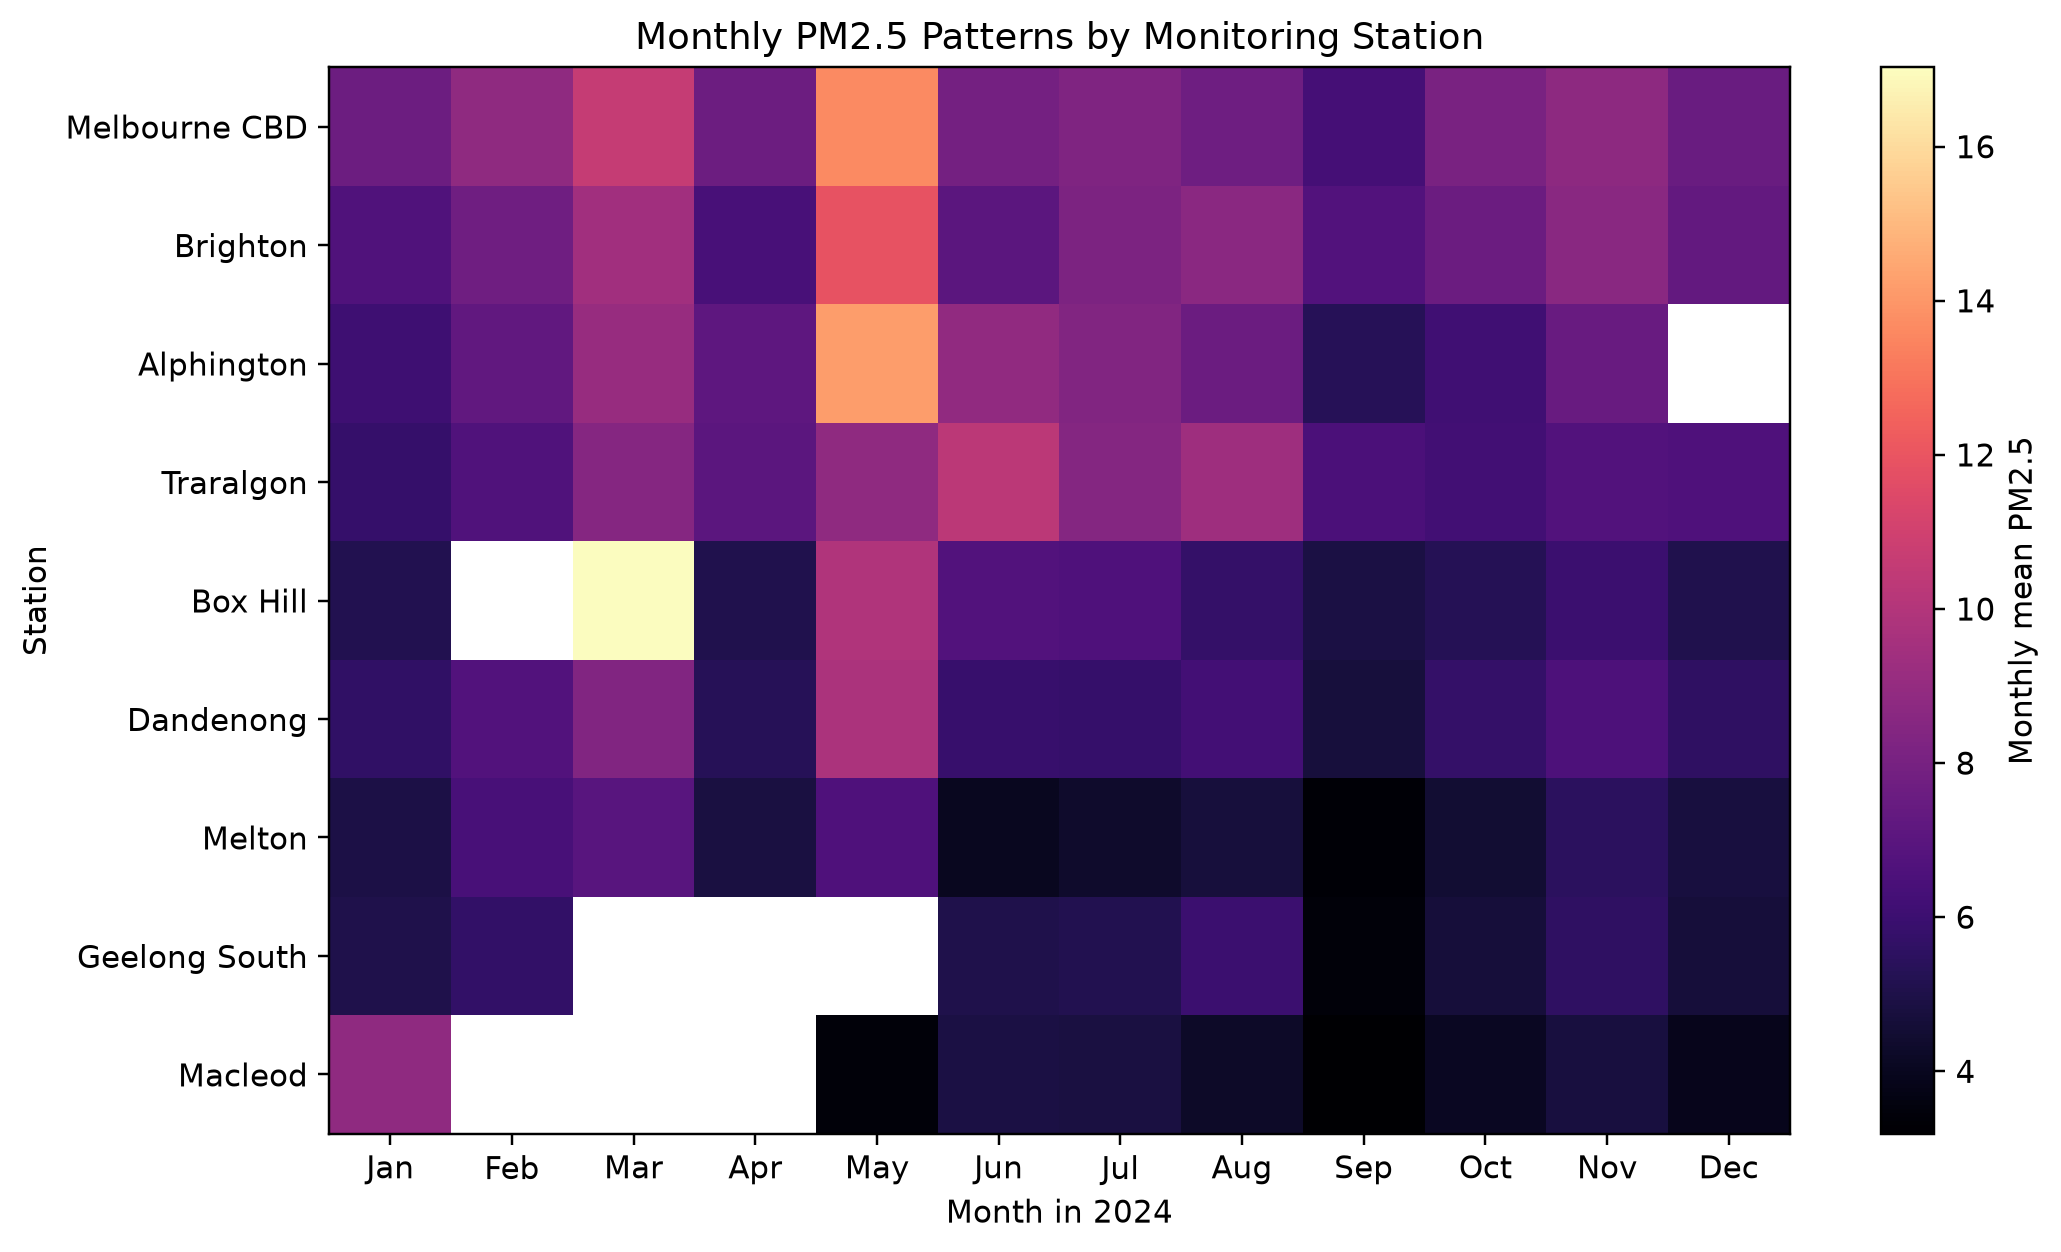
\includegraphics[width=0.92\textwidth]{fig01_monthly_pm25_heatmap.png}
  \caption{Monthly PM2.5 patterns by monitoring station.}
\end{figure}

The monthly heatmap shows that PM2.5 exposure was not evenly distributed across the year. Several metropolitan stations show a clear April-May elevation, while Traralgon also shows a winter increase. This supports a reading in which short smoke events, traffic, local residential heating and regional accumulation all matter, rather than a single seasonal explanation.

\begin{figure}[H]
  \centering
  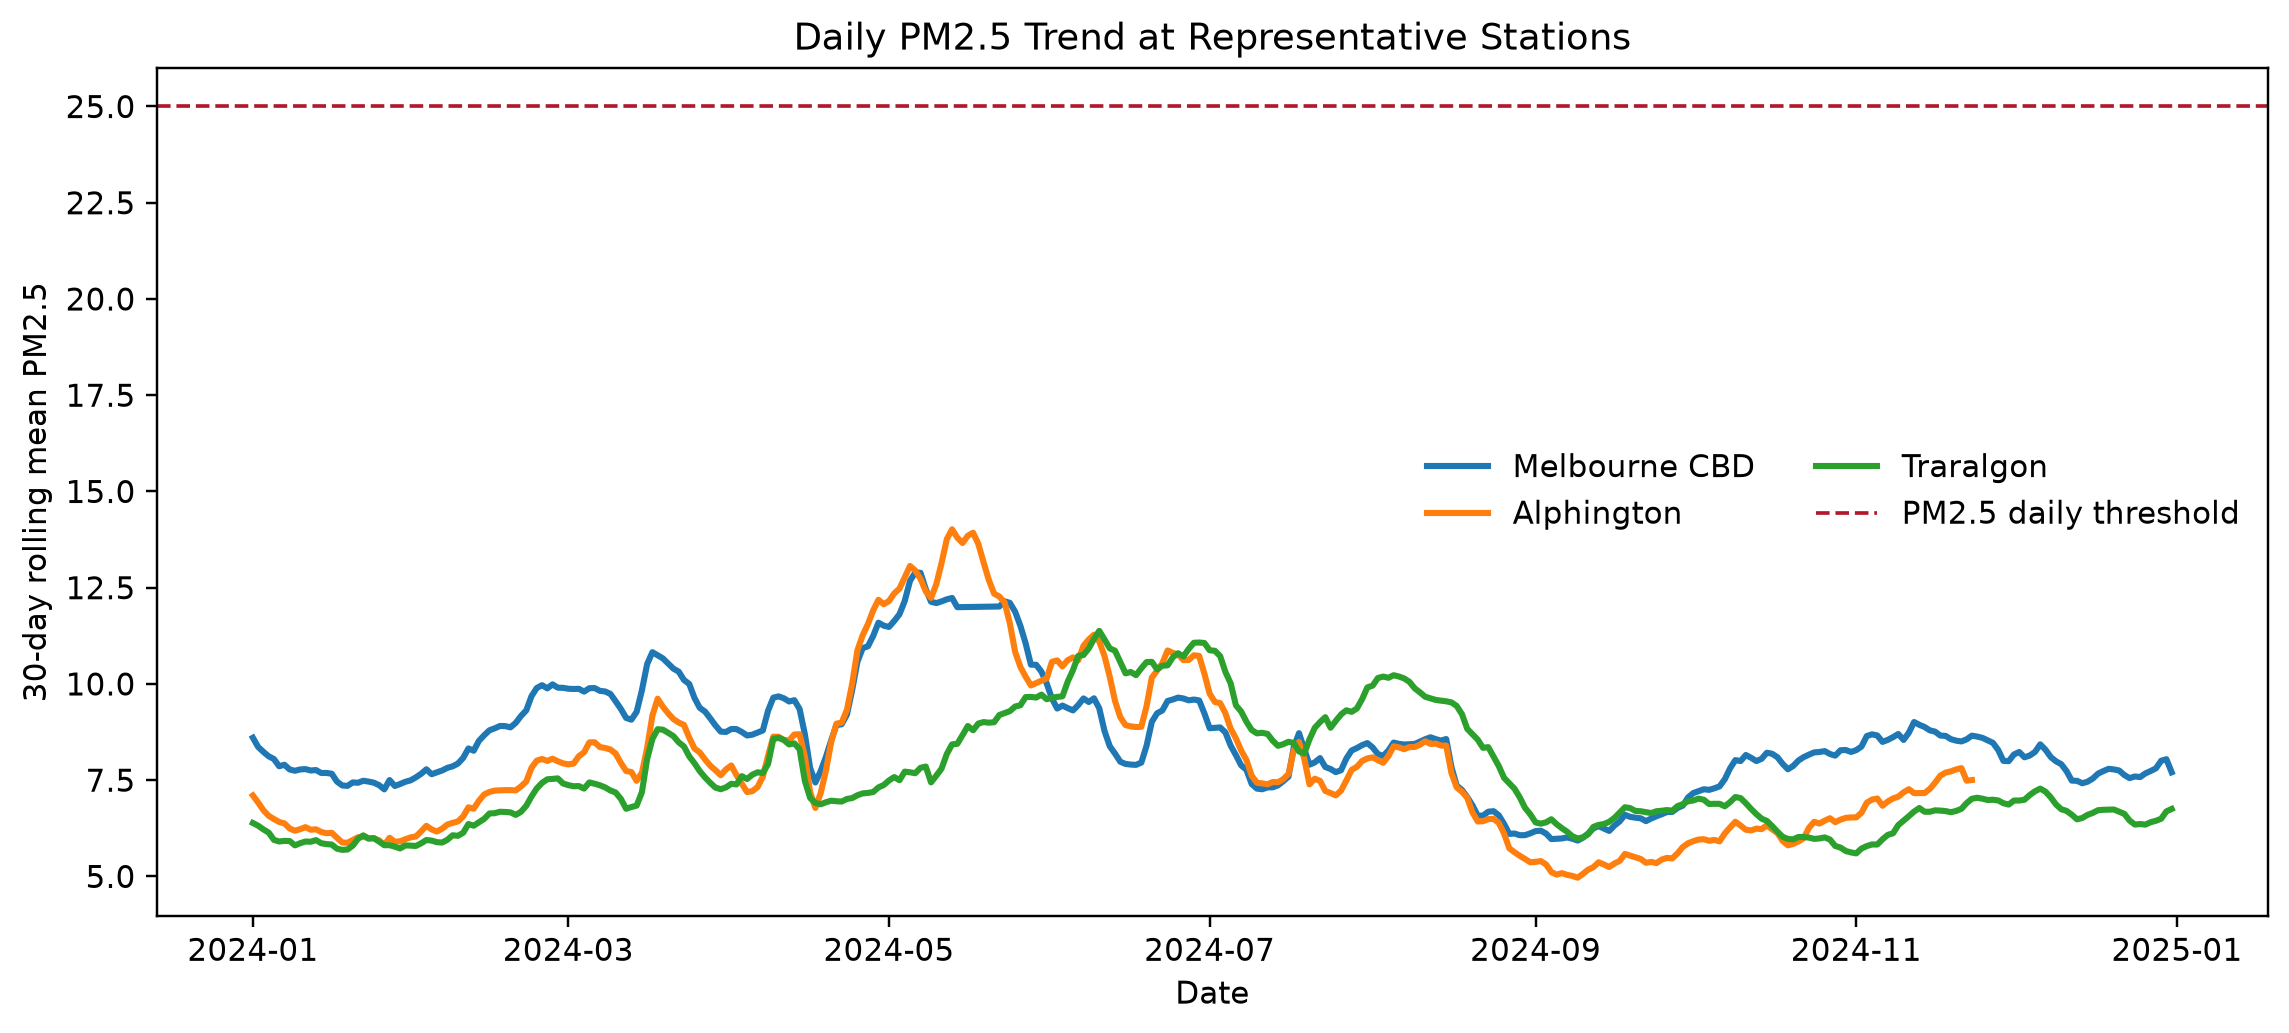
\includegraphics[width=0.92\textwidth]{fig02_daily_pm25_timeseries.png}
  \caption{Daily PM2.5 trend at representative stations.}
\end{figure}

The daily time-series view reinforces the same point. Representative stations do not move identically: Melbourne CBD, Alphington and Traralgon have different baselines and different episodes of elevated PM2.5.

\begin{figure}[H]
  \centering
  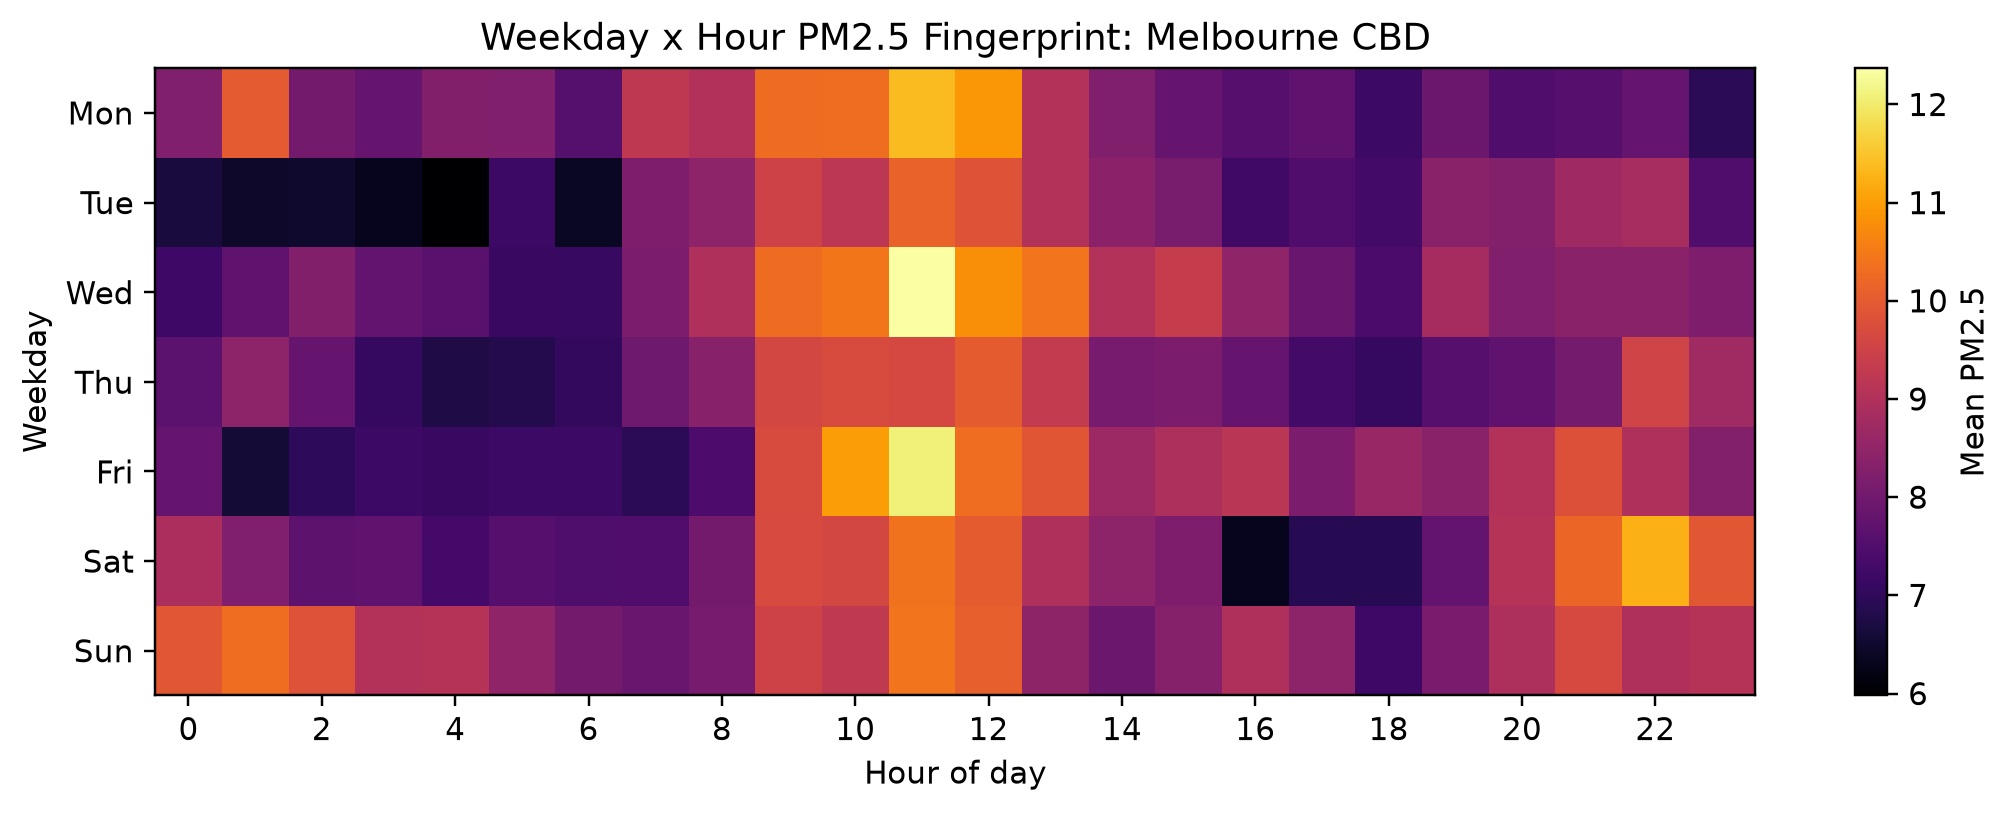
\includegraphics[width=0.88\textwidth]{fig03_weekday_hour_pm25.png}
  \caption{Weekday-hour PM2.5 fingerprint.}
\end{figure}

The weekday-hour fingerprint highlights daily rhythm. A station such as Melbourne CBD tends to show a weekday daytime pattern consistent with traffic and activity, while residential stations can show different evening or weekend signatures.

\section{Pollutant Differences and Exceedances}

\begin{figure}[H]
  \centering
  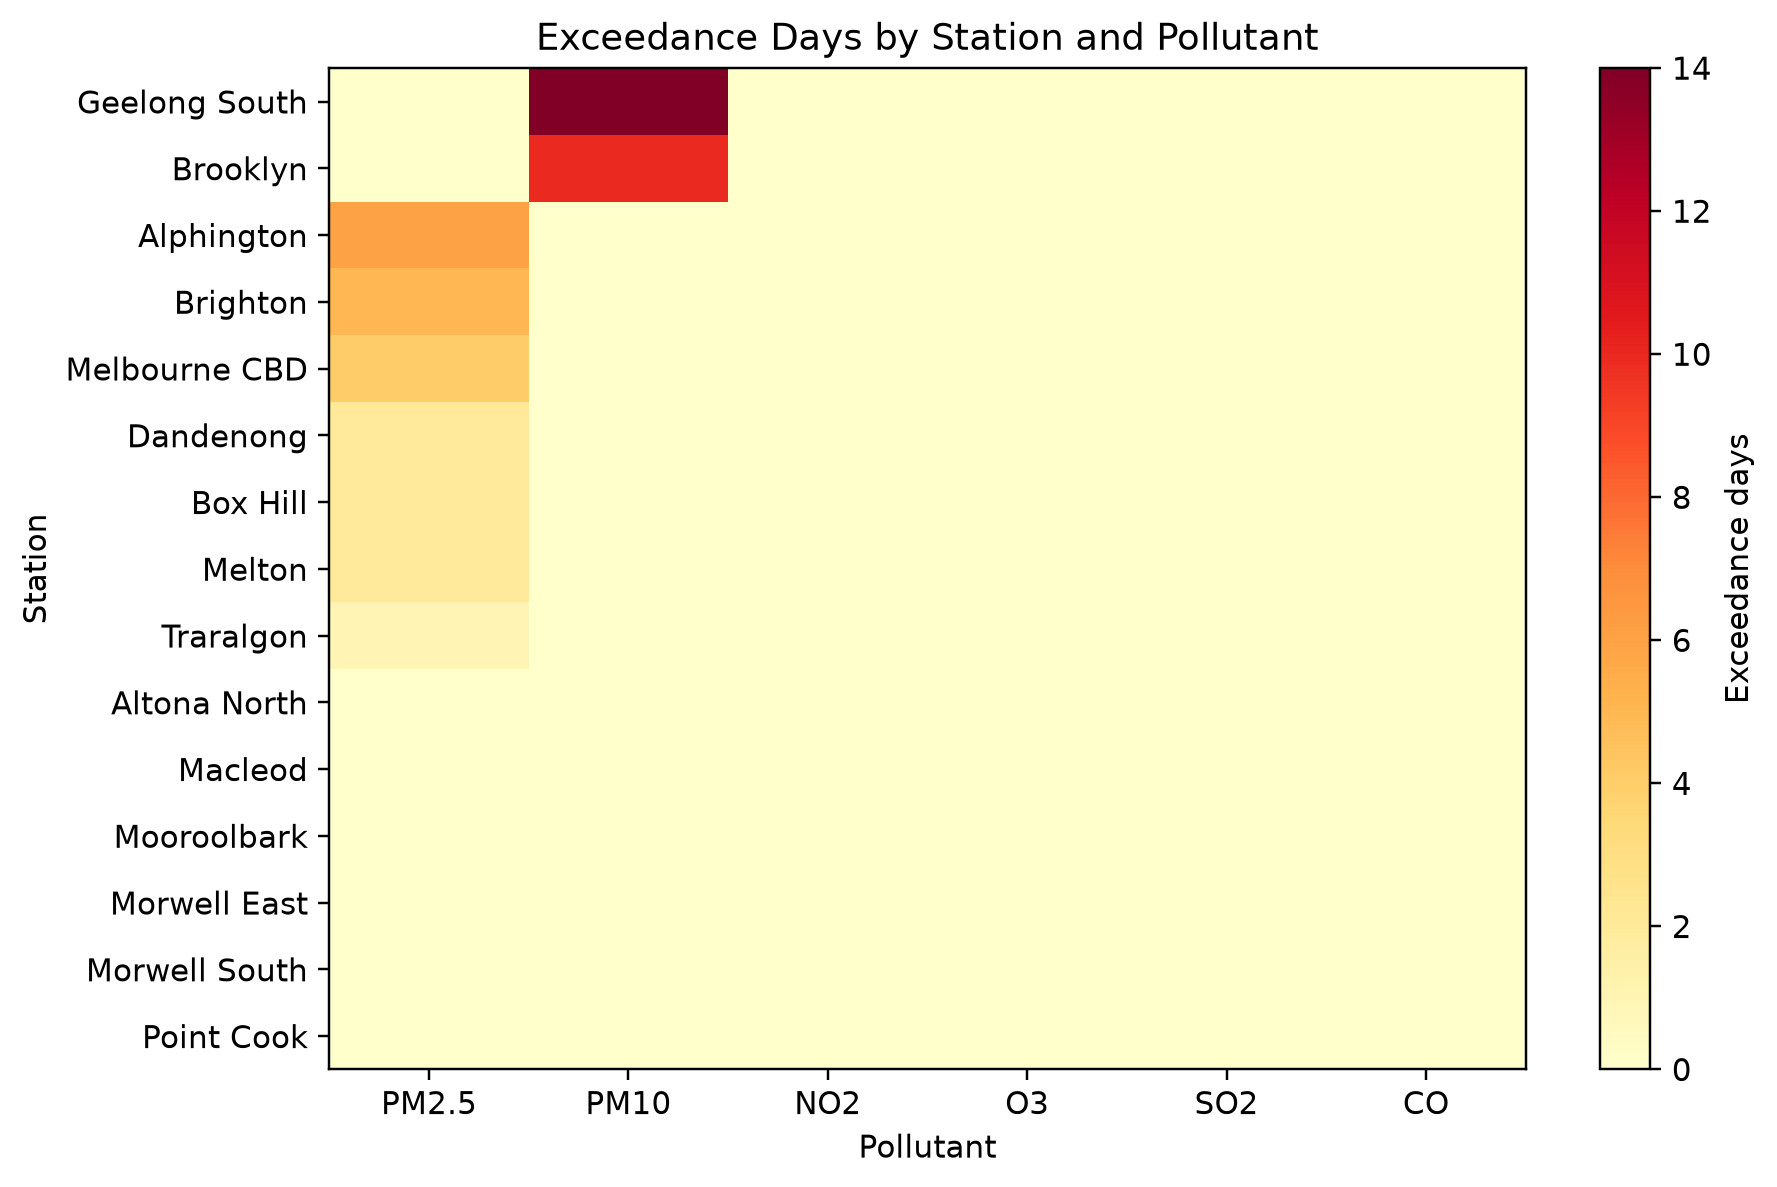
\includegraphics[width=0.82\textwidth]{fig04_exceedance_heatmap.png}
  \caption{Exceedance days by station and pollutant.}
\end{figure}

Exceedance counts are concentrated in particulate matter. PM10 exceedances are highest at Geelong South and Brooklyn, while PM2.5 exceedances are highest at Alphington, Brighton and Melbourne CBD. In the processed 2024 dataset, NO2, O3, SO2 and CO exceedance counts are zero under the thresholds used in this workflow. This suggests that the regulatory story in this dataset is driven mainly by particulate matter, but with PM2.5 and PM10 pointing to different sites and likely different sources.

\section{Exposure and Socio-economic Context}

\begin{figure}[H]
  \centering
  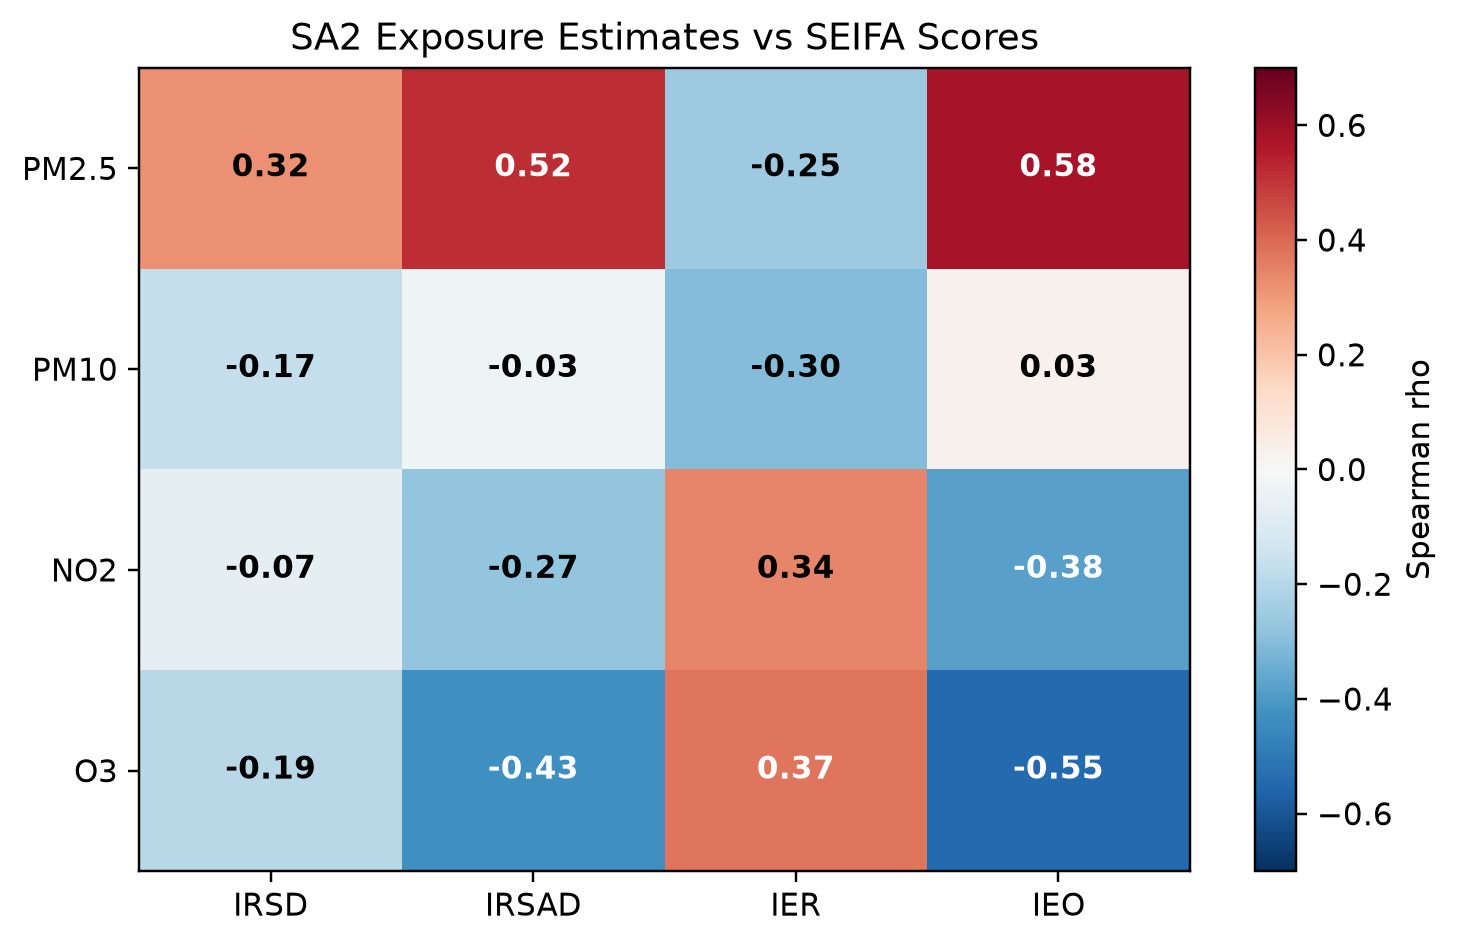
\includegraphics[width=0.82\textwidth]{fig05_seifa_correlation_heatmap.png}
  \caption{SA2 exposure estimates vs SEIFA scores.}
\end{figure}

The correlation heatmap compares IDW-estimated annual exposure values with four SEIFA dimensions at SA2 level. Higher SEIFA scores generally mean less disadvantage. PM2.5 has positive correlations with IRSD, IRSAD and IEO, including a strong positive relationship with IEO. In plain terms, the modelled annual PM2.5 surface is higher in some higher-education and higher-occupation inner-city areas. PM10 is more weakly related to SEIFA except for a negative relationship with economic resources. NO2 and O3 show stronger negative relationships with IEO, which is closer to a conventional environmental-justice pattern.

\begin{figure}[H]
  \centering
  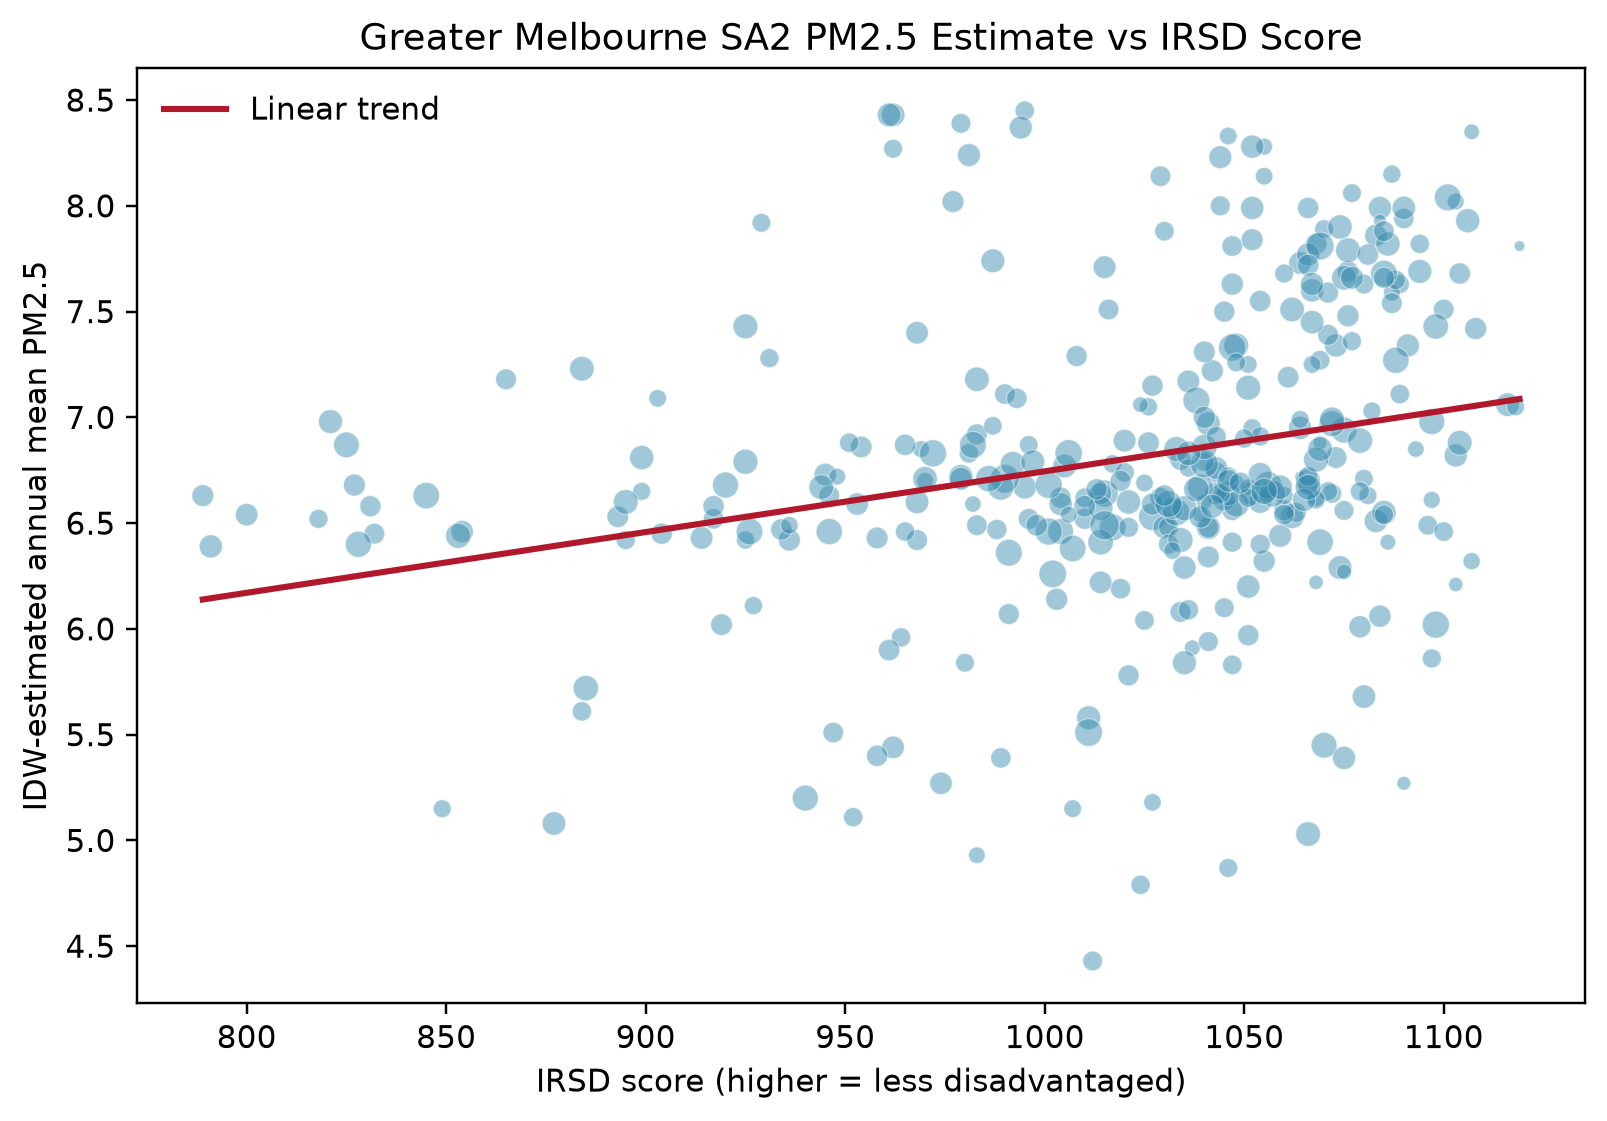
\includegraphics[width=0.82\textwidth]{fig06_pm25_irsd_scatter.png}
  \caption{PM2.5 estimate vs IRSD score.}
\end{figure}

The PM2.5-IRSD scatterplot shows why the result should be interpreted carefully. PM2.5 is not simply highest in the most disadvantaged areas. Inner-city geography, traffic density, urban form and monitoring-station distribution shape the annual exposure estimate. This does not mean socio-economic inequality is absent; it means that the direction and strength of the relationship depend on pollutant, SEIFA dimension and spatial scale.

\section{Main Findings}

\begin{itemize}[leftmargin=*]
  \item PM2.5 exposure has strong temporal structure, including an April-May elevation at several urban stations.
  \item PM10 exceedances are concentrated at Geelong South and Brooklyn, suggesting a different source story from PM2.5.
  \item Weekday-hour patterns show that station-level exposure has interpretable daily rhythms.
  \item The Greater Melbourne PM2.5-SEIFA relationship is not monotonic; higher modelled PM2.5 appears in some relatively advantaged inner areas.
  \item NO2 and O3 show more conventional negative relationships with education/occupation-related SEIFA scores.
  \item Any environmental-equity conclusion must be pollutant-specific and scale-aware.
\end{itemize}

\section{Limitations}

This project uses a single year of monitoring data. The spatial surface is an IDW estimate from a limited number of metropolitan stations and should not be interpreted as street-level exposure. SA2 averages also hide within-area variation, especially near roads, industrial sites and local heating sources. The results are best treated as an exploratory association analysis, not causal evidence.

\section{Reproducibility}

The project is organised into \texttt{code}, \texttt{data}, \texttt{figures}, \texttt{outputs} and \texttt{report} folders. The workflow does not require network access once the three raw source files are placed in \texttt{data/raw}. The main commands are:

\begin{verbatim}
python3 -m pip install -r requirements.txt
python3 code/01_check_data.py
python3 code/02_build_processed_data.py
python3 code/03_make_figures.py
latexmk -cd -xelatex -interaction=nonstopmode \
  -jobname=air_quality_report report/report.tex
\end{verbatim}

\section*{References}

\begin{itemize}[leftmargin=*]
  \item EPA Victoria / DataVic. \href{https://discover.data.vic.gov.au/dataset/epa-air-watch-all-sites-air-quality-hourly-averages-yearly}{EPA AirWatch all sites air quality hourly averages yearly}.
  \item Australian Bureau of Statistics. \href{https://www.abs.gov.au/statistics/people/people-and-communities/socio-economic-indexes-areas-seifa-australia/2021}{Socio-Economic Indexes for Areas (SEIFA), Australia, 2021}.
  \item Australian Bureau of Statistics. \href{https://www.abs.gov.au/statistics/standards/australian-statistical-geography-standard-asgs-edition-3/jul2021-jun2026/access-and-downloads/digital-boundary-files}{Australian Statistical Geography Standard (ASGS) Edition 3 digital boundary files}.
  \item Shepard, D. (1968). A two-dimensional interpolation function for irregularly-spaced data.
\end{itemize}

\end{document}
